\chapter{神完全的憤怒施行公義審判（15:1-16:21）}

如果說前面的七印與七號讓我們逐步看見神的審判，那麼到了啟示錄第15、16章，審判進入最後的階段。約翰看見七位天使掌管末了的七災，並將七個金碗盛滿神的忿怒，傾倒在地上。

在可怕的審判之前，約翰先讓我們看見一幅得勝的畫面：那些勝過獸、勝過獸的像和牠名字數目的人，站在玻璃海上，手拿著神的琴，唱著「摩西的歌，又唱羔羊的歌」。這個安排非常重要。審判臨到之前，約翰先讓我們看見得勝的教會。屬於羔羊的人不是在神的忿怒之下，而是在祂的保守中。他們經過患難，卻並沒有向獸屈服，所以最終站在神面前歡喜的敬拜祂。

\section{唱羔羊的新歌}

\begin{ScriptureBox2}{圈出站在玻璃海上的人手裡拿著什麼，以及他們唱的是誰的歌。劃出15:3中描述神的作為和道途的字句。}
\item[15:1] 我又看見在天上有異象、大而且奇、就是七位天使掌管末了的七災．因為　神的大怒在這七災中發盡了。

\item[15:2] 我看見彷彿有玻璃海、其中有火攙雜．又看見那些勝了獸和獸的像、並他名字數目的人、都站在玻璃海上、拿著　神的琴．

\item[15:3] 唱　神僕人摩西的歌、和羔羊的歌、說、主　神、全能者阿、你的作為大哉、奇哉、萬世之王阿、〔世或作國〕你的道途義哉、誠哉。

\item[15:4] 主阿、誰敢不敬畏你、不將榮耀歸與你的名呢．因為獨有你是聖的．萬民都要來在你面前敬拜．因你公義的作為已經顯出來了。

\item[15:5] 此後、我看見在天上那存法櫃的殿開了．

\item[15:6] 那掌管七災的七位天使、從殿中出來、穿著潔白光明的細麻衣、〔細麻衣有古卷作寶石〕胸間束著金帶。

\item[15:7] 四活物中有一個把盛滿了活到永永遠遠之　神大怒的七個金碗給了那七位天使。

\item[15:8] 因　神的榮耀、和能力、殿中充滿了煙．於是沒有人能以進殿、直等到那七位天使所降的七災完畢了。
\end{ScriptureBox2}

\begin{InDepth}
\InDepthHeading{摩西的歌與羔羊的歌}

啟示錄15章與出埃及記15章有明顯對照。如表\ref{tab:rev_exdus_15}。當摩西與百姓過紅海，法老及埃及軍隊被淹沒在紅海裡。摩西與百姓雀躍，唱新歌。到了啟示錄15章，是羔羊救贖祂的百姓、勝過一切敵對勢力的終極勝利之歌。

\par\medskip\noindent
\begin{minipage}{\linewidth}
\centering\small
\renewcommand{\arraystretch}{1}\setlength{\tabcolsep}{4pt}
\captionof{table}{啟示錄15章與出埃及記15章}
\label{tab:rev_exdus_15}
\begin{tabularx}{\linewidth}{@{}>{\raggedright\arraybackslash}X
                               >{\raggedright\arraybackslash}X
                               >{\raggedright\arraybackslash}X@{}}
\hline
啟示錄15 & 出埃及15 & 內容 \\
\hline
1 七災 & 埃及十災 & 神對仇敵施行審判 \\
2 站在玻璃海上 & 過紅海 & 神拯救祂的百姓 \\
2 獸 & 法老及埃及軍隊 & 神與仇敵爭戰 \\
3 摩西的歌 & 摩西的歌 & 救贖後的勝利之歌 \\
5 存法櫃的殿 & 會幕／聖所 & 神的同在 \\
8 煙充滿殿 & 神的榮耀 & 神臨在並施行審判 \\
\hline
\end{tabularx}
\end{minipage}
\end{InDepth}

這歌唱的不是稱讚人的勇敢，而是宣告神的作為「大哉、奇哉」、「義哉、誠哉」。我們在患難中容易把注意力放在自己的處境上，這首歌使我們的眼目重新定睛在神身上。

\begin{ReaderQuestion}
啟示錄15:3-4的歌頌不是稱讚人的勇敢，而是宣告神的作為「大哉、奇哉」、「義哉、誠哉」。我們在患難中容易把注意力放在自己的處境上，這首歌如何把我們的眼目重新轉向神？
\end{ReaderQuestion}

天使接了碗去傾倒在地上。地上有災，天上有殿，直到七位天使所降的七災完畢了。

\section{第1-5碗}

\begin{figure}[htbp]
    \centering
    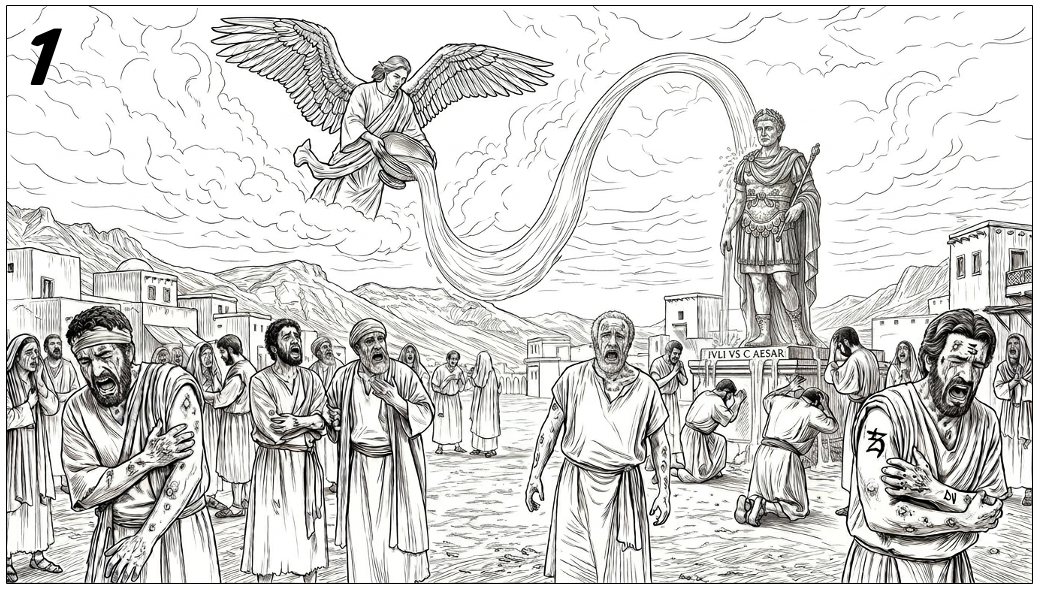
\includegraphics[
    width=1\textwidth, 
    trim=0 0 0 0, 
    clip]{images/bowl_1.png}
\end{figure}


\begin{figure}[htbp]
    \centering
    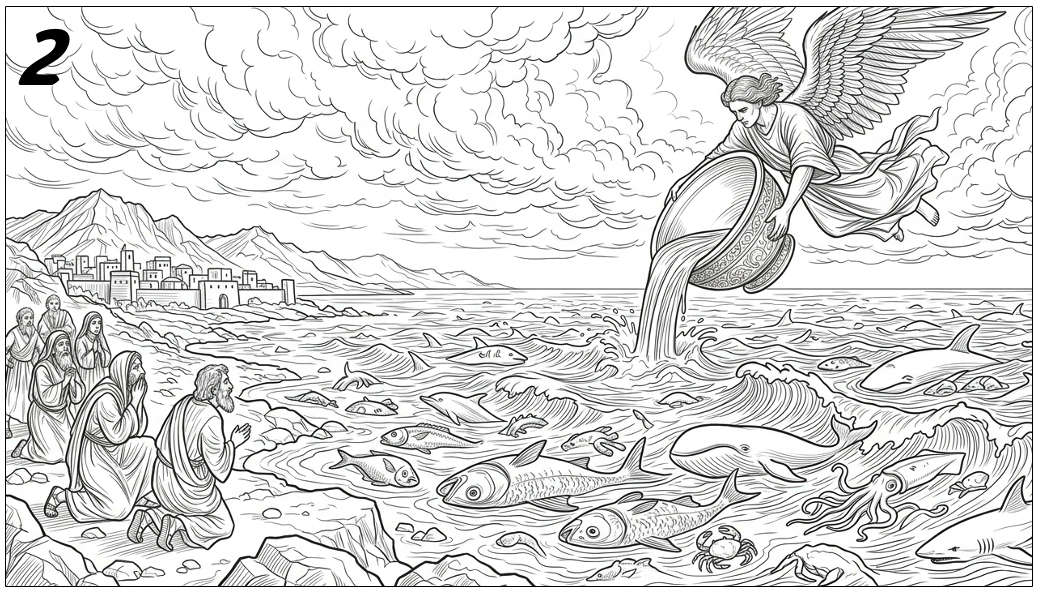
\includegraphics[
    width=1\textwidth, 
    trim=0 0 0 0, 
    clip]{images/bowl_2.png}
\end{figure}


\begin{ScriptureBox2}{前五碗各倒在哪裡？劃出16:9和16:11中人的反應。}

\item[16:1] 我聽見有大聲音從殿中出來、向那七位天使說、你們去、把盛　神大怒的七碗倒在地上。

\item[16:2] 第一位天使便去、把碗倒在地上、就有惡而且毒的瘡、生在那些有獸印記、拜獸像的人身上。

\item[16:3] 第二位天使把碗倒在海裡、海就變成血、好像死人的血．海中的活物都死了。

\item[16:4] 第三位天使把碗倒在江河與眾水的泉源裡、水就變成血了。

\item[16:5] 我聽見掌管眾水的天使說、昔在今在的聖者阿、你這樣判斷是公義的．

\item[16:6] 他們曾流聖徒與先知的血、現在你給他們血喝．這是他們所該受的。

\item[16:7] 我又聽見祭壇中有聲音說、是的、主　神、全能者阿、你的判斷義哉、誠哉。

\item[16:8] 第四位天使把碗倒在日頭上、叫日頭能用火烤人。

\item[16:9] 人被大熱所烤、就褻瀆那有權掌管這些災的　神之名、並不悔改將榮耀歸給　神。

\item[16:10] 第五位天使把碗倒在獸的座位上、獸的國就黑暗了．人因疼痛就咬自己的舌頭．

\item[16:11] 又因所受的疼痛、和生的瘡、就褻瀆天上的　神、並不悔改所行的。

\end{ScriptureBox2}

\begin{figure}[htbp]
    \centering
    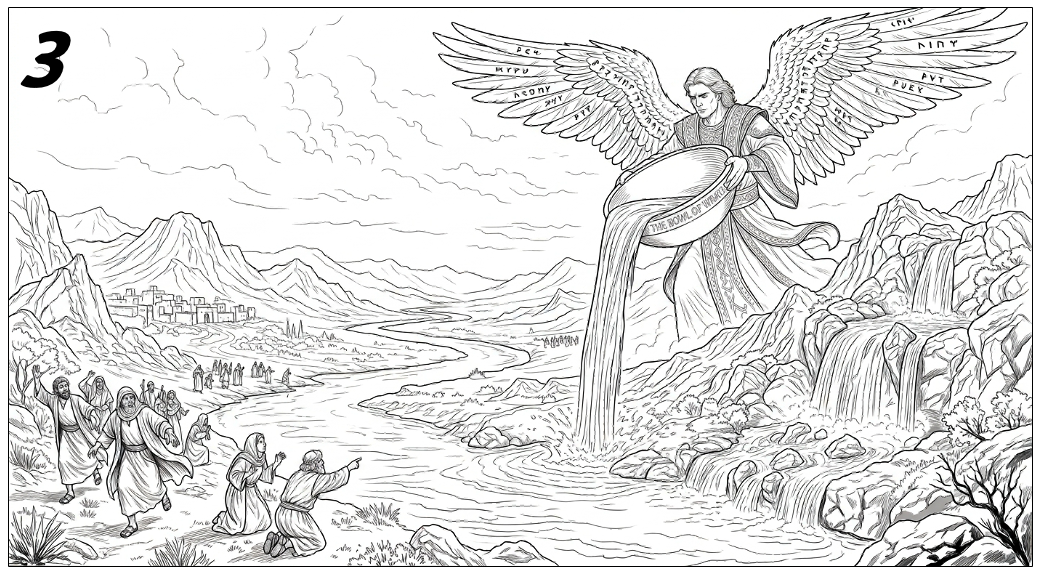
\includegraphics[
    width=1\textwidth, 
    trim=0 0 0 0, 
    clip]{images/bowl_3.png}
\end{figure}


第一碗臨到拜獸的人，第二、三碗擊打海洋與江河，第四、五碗擴大到人與獸的國，第六碗聚集末後爭戰，第七碗宣告「成了」，七碗的審判一步一步加重，直到神的忿怒完全傾倒，審判達到終局。

這些可怕的場景，不是發生在那些屬於羔羊、蒙祂救贖的人身上，而是臨到「那些有獸印記、拜獸像的人」。每一個碗都盛滿了神完全的忿怒。神曾經長久忍耐，一次又一次呼召人悔改。然而到了這裡，時間已經到了。

\begin{ReaderQuestion}
你如何理解「神的忍耐」與「神最終的審判」之間的關係？神的忍耐是否代表祂輕看罪？
\end{ReaderQuestion}


\begin{figure}[htbp]
    \centering
    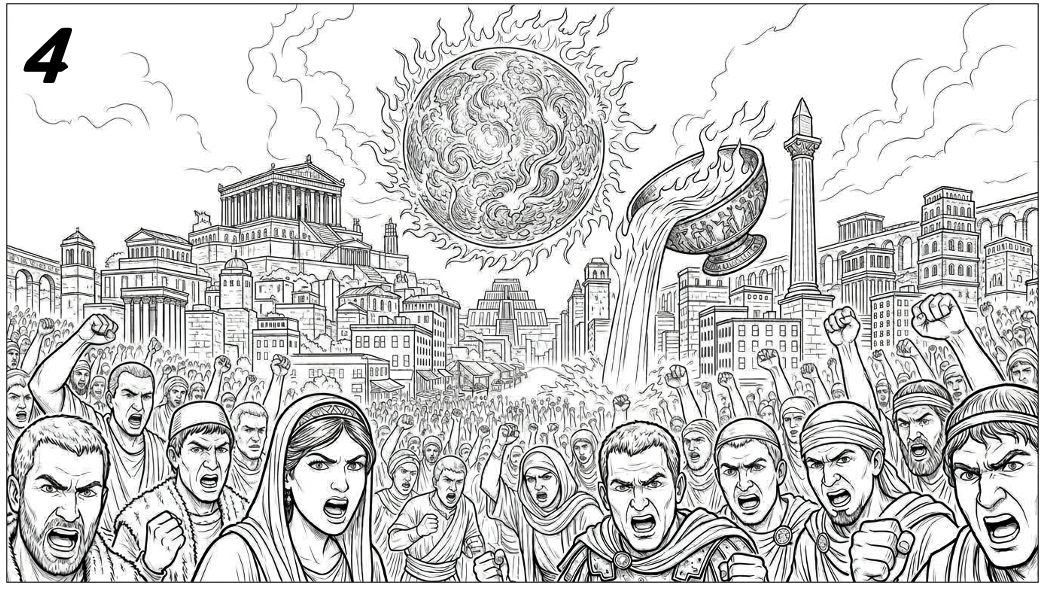
\includegraphics[
    width=1\textwidth, 
    trim=0 0 0 0, 
    clip]{images/bowl_4.png}
\end{figure}

讀到這裡，我們會想起第一冊《被恩典追上》第十章所介紹的愛德華滋（Jonathan Edwards）著名講道〈在忿怒之神手中的罪人〉（\textit{Sinners in the Hands of an Angry God}）。愛德華滋以極其強烈的語言描述尚未投靠基督的罪人所面對的危險：
\begin{quote}
「罪人啊！當仔細思量你所處可怕的危險：那是烈怒的大熔爐，寬闊無底的深淵，充滿火焰與怒氣，而你被握在那位神的手中，他對你的怒氣如同已經激怒的烈火，如同眾多地獄中的罪人一樣猛烈。你懸於纖細的線上，神聖的怒火焰環繞其周，每一刻都準備焚燒它；你沒有任何中保的幫助，無法挽救自己，無法抵禦怒火，一切自身所有、一切行為，都不能使神寬恕你一刻……」
\end{quote}

親愛的讀者，今天仍是恩典的日子。羔羊已經為罪人捨命。正因為將來的審判如此真實，神的恩典才顯得如此寶貴。你願意回應神的恩典，接受祂的救恩嗎？

\begin{ReaderQuestion}
今天仍是恩典的日子。你認為自己應當如何更認真地悔改、持守信仰、仰望羔羊，並向還沒有認識基督的人傳福音？
\end{ReaderQuestion}

\begin{figure}[htbp]
    \centering
    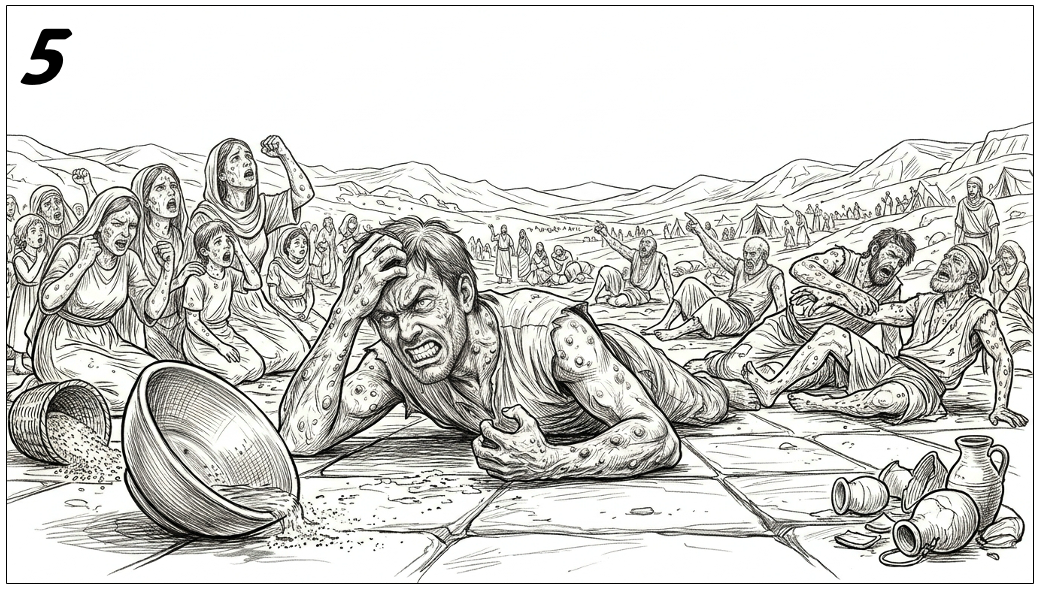
\includegraphics[
    width=1\textwidth, 
    trim=0 0 0 0, 
    clip]{images/bowl_5.png} 
\end{figure}


\section{第六碗}

\begin{ScriptureBox2}{三個污穢的靈從誰的口中出來？他們聚集眾王要做什麼？耶穌在16:15說了什麼祝福？}

\item[16:12] 第六位天使把碗倒在伯拉大河上、河水就乾了、要給那從日出之地所來的眾王預備道路。

\item[16:13] 我又看見三個污穢的靈、好像青蛙、從龍口獸口並假先知的口中出來．

\item[16:14] 他們本是鬼魔的靈、施行奇事、出去到普天下眾王那裡、叫他們在　神全能者的大日聚集爭戰。

\item[16:15] （看哪、我來像賊一樣。那儆醒、看守衣服、免得赤身而行、叫人見他羞恥的、有福了。）

\item[16:16] 那三個鬼魔便叫眾王聚集在一處、希伯來話叫作「哈米吉多頓。」

\end{ScriptureBox2}

\begin{figure}[htbp]
    \centering
    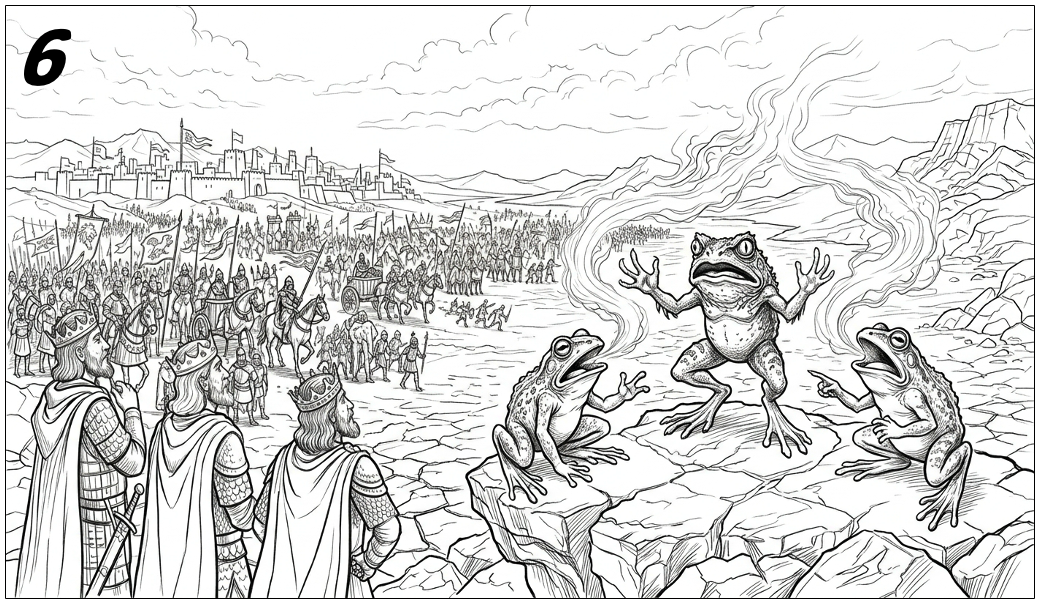
\includegraphics[
    width=1\textwidth, 
    trim=0 0 0 0, 
    clip]{images/bowl_6.png} 
\end{figure}


這一節是七碗審判的高潮之一。
從龍、獸和假先知口中出來、形狀像青蛙的三個污穢的靈，唆使世上的君王聚集。這些列國的君王以為自己正在作自己的政治與軍事決定，然而約翰從屬靈的角度看見，他們受到邪靈的迷惑，正被聚集到神最後的審判之中。

「哈米吉多頓」(Armageddon)在許多末世小說與電影中被當做末日大戰的場景。這個名稱通常與希伯來文的米吉多（Megiddo）有關。
米吉多是古代以色列的重要戰略地區，也是多場戰爭的所在地。因此很自然成為約翰描寫末日衝突的象徵性背景。

啟示錄 16:16 描述敵對神的地上勢力被唆使聚集到「哈米吉多頓」，而真正的哈米吉多頓戰役場景是在後面的 啟示錄 19:19–21。此哈米吉多頓戰役也不是兩個勢均力敵的陣營，是基督完全得勝。
\begin{InDepth}
\InDepthHeading{啟示錄16章與19章的關聯}

因為經文橫跨兩章，我用圖\ref{rev_16_19_armageddon_chinese}表示。此圖也使我們看到，是撒旦透過三隻污穢的青蛙，唆使隨從他的人類來攻擊神。只是他也知道「自己的時候不多、就氣忿忿的下到你們那裡去了。」（啟示錄12:12）

\par\medskip\noindent
\begin{minipage}{\linewidth}
\centering
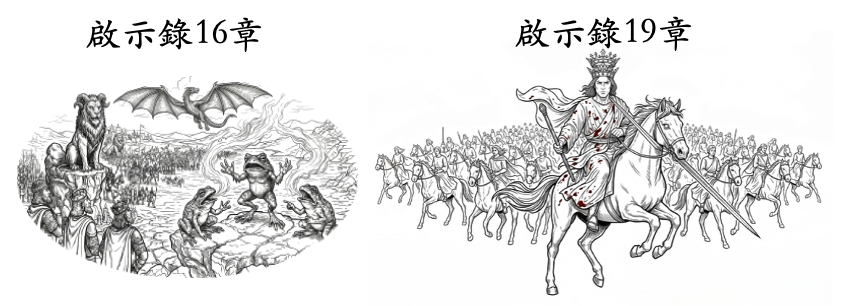
\includegraphics[
    width=\linewidth,
    trim=0 10 20 0,
    clip]{images/rev_16_19_armageddon_chinese.png}
\captionof{figure}{哈米吉多頓的戰役}
\label{rev_16_19_armageddon_chinese}
\end{minipage}
\end{InDepth}

\section{第七碗}

\begin{ScriptureBox2}{寶座上的大聲音宣告什麼？圈出接著發生的每一個現象，並留意人對雹災的反應。}

\item[16:17] 第七位天使把碗倒在空中、就有大聲音從殿中的寶座上出來、說、成了．

\item[16:18] 又有閃電、聲音、雷轟、大地震、自從地上有人以來、沒有這樣大這樣利害的地震。

\item[16:19] 那大城裂為三段、列國的城也都倒塌了．　神也想起巴比倫大城來、要把那盛自己烈怒的酒杯遞給他。

\item[16:20] 各海島都逃避了、眾山也不見了。

\item[16:21] 又有大雹子從天落在人身上、每一個約重一他連得．〔一他連得約有九十斤〕為這雹子的災極大、人就褻瀆　神。

\end{ScriptureBox2}

這裡最重要的是神說「成了」。神的審判已經完成，但人的悖逆直到最後仍然沒有改變。

這樣的地震，是有人類以來，沒有經歷過的地震。雹重90斤，約是45公斤，或是100英鎊。
但人仍然「褻瀆神」。

讀到這裡，讓我們想起第一冊「被恩典追上」12章曾經引用魯益師（C.S. Lewis）在其著作《大分裂》說的：
\begin{quote}
「到最後，人只分為兩種：一種是對神說「願你的旨意成就」的人。另一種是最後由神對他們說「願你的己意成就」的人。」—魯益師（C.S. Lewis）\footnote{“There are only two kinds of people in the end: those who say to
God, ”Thy will be done,” and those to whom God says, in the end,
”Thy will be done.” All that are in Hell, choose it. Without that
self-choice there could be no Hell. No soul that seriously and
constantly desires joy will ever miss it. Those who seek find. Those
who knock it is opened.” Lewis, C. S. (1946). \textit{The great divorce.}
Geoffrey Bles.}
\end{quote}

\begin{ReaderQuestion}
魯益師說，到最後人只分為兩種：一種是對神說「願你的旨意成就」的人，另一種是最後由神對他們說「願你的己意成就」的人。在你生命中的哪一個領域，你仍然緊抓著自己的意思？今天對神說「願你的旨意成就」，會是什麼樣子？
\end{ReaderQuestion}

\section*{七碗的特徵}

{
\small
\renewcommand{\arraystretch}{1}
\begin{longtable}{p{1.5cm} p{2cm} p{2cm}}
\caption{七碗審判口訣}
\label{tab:seven-bowls-zh} \\
\hline
碗 & 經文 & 審判 \\
\hline
\endfirsthead

\multicolumn{3}{l}{\small\itshape 表~\thetable（續）} \\
\hline
碗 & 經文 & 審判 \\
\hline
\endhead

\hline
\endfoot

\hline
\endlastfoot

第一碗 & 16:1--2 & 惡毒瘡 \\
第二碗 & 16:3 & 海變血 \\
第三碗 & 16:4--7 & 河變血 \\
第四碗 & 16:8--9 & 日火烤 \\
第五碗 & 16:10--11 & 痛咬舌 \\
第六碗 & 16:12--16 & 集爭戰 \\
第七碗 & 16:17--21 & 成了 \\
\end{longtable}
}
